\documentclass[a4paper, 12pt]{article}

\usepackage[spanish]{babel}
\usepackage{amsmath}
\usepackage{hyperref}
\usepackage{graphicx, listings, xcolor, subcaption,caption}

\definecolor{codegreen}{rgb}{0,0.6,0}
\definecolor{codegray}{rgb}{0.5,0.5,0.5}
\definecolor{codepurple}{rgb}{0.58,0,0.82}
\definecolor{backcolour}{rgb}{0.95,0.95,0.92}
\lstdefinestyle{mystyle}{
    backgroundcolor=\color{backcolour},   
    commentstyle=\color{codegreen},
    keywordstyle=\color{magenta},
    numberstyle=\tiny\color{codegray},
    stringstyle=\color{codepurple},
    basicstyle=\ttfamily\footnotesize,
    breakatwhitespace=false,         
    breaklines=true,                 
    captionpos=b,                    
    keepspaces=true,                 
    numbers=left,                    
    numbersep=5pt,                  
    showspaces=false,                
    showstringspaces=false,
    showtabs=false,                  
    tabsize=2
}

\setlength{\parskip}{8pt}
\setlength{\parindent}{0pt}
\lstset{style=mystyle, language=Python}
\renewcommand{\arraystretch}{1.5}

\title{\vspace{-3cm}Tarea 1: Procesamiento Digital de Imágenes}
\author{
    Angel de Jesús Maldonado Juárez\\
    Universidad Autónoma de San Luis Potosí\\
    Facultar de Ingeniería - Ing. En Sistemas Inteligentes\\
    \textbf{Materia:} Visión Computacional\\
    \textbf{Prof:} Dr. César Augusto Puente Montejano\\
    \textbf{Autor:} Angel de Jesús Maldonado Juárez
}
\date{\textbf{Fecha de entrega:} lunes 12 de septiembre de 2022}

\begin{document}
\maketitle

\begin{center}
    \rule{\textwidth}{0.5pt}
    \begin{abstract}
        ...
    \end{abstract}
    \rule{\textwidth}{0.5pt}
\end{center}

\section{Transformaciones Geométricas}
Las \emph{transformaciones geométricas} son una "manipulación" de la información de una entidad que puede ser representada en un \emph{espacio geométrico} como lo pueden ser sus \textbf{coordenadas}. En el contexto de una imagen se considera que al aplicar alguna transformación, también se transforma el \emph{sistema de coordenadas} de la imagen; en una \textbf{transformación espacial} cada punto $(x,y)$ de una imagen $A$, es \textbf{mapeado} a un punto $(u,v)$ en un nuevo \emph{sistema de coordenadas}.

Para aplicar transformaciones a una imagen, se tiene que multiplicar la \emph{matriz de transformación} a cada par de coordenadas de la imagen, existen varios tipos de transformaciones, cada una se describe con su propia matriz. Las más comunes son: \emph{traslación}, \emph{rotación}, \emph{escalado}, y \emph{shearing} (recorte o ajuste). La principal tarea de estas transformaciones es mapear cada punto $(x,y)$ de la imagen a una nueva posición o punto $(u,v)$, con base a los parámetros que se hayan definido en la transformación.

También existen transformaciones más complejas que se caracterizan por aplicar más transformaciones en su proceso: \emph{transformación rígida} (traslación + rotación), \emph{transformación de similitud} (traslación + rotación + escalado), \emph{transformación de afinamiento} (traslaciones + rotaciones + escalado + shearing).

En este reporte se aplica una transformación de \emph{rotación} a determinada imagen, por lo que para obtener las nuevas coordenadas $(u,v)$ de cada pixel la imagen se realiza lo siguiente:

\begin{equation}
    \begin{bmatrix}
        u \\
        v
    \end{bmatrix}
    =
    \begin{bmatrix}
        cos\theta & -sen\theta \\
        sen\theta & cos\theta
    \end{bmatrix}
    *
    \begin{bmatrix}
        x \\
        y
    \end{bmatrix}
\end{equation}

Donde, $[u,v]$ son las nuevas coordenadas para cada pixel de la imagen calculada multiplicando la matriz de rotación (1) por el par de coordenadas $[x,y]$, y $\theta$ es el ángulo de rotación de la imagen.

\section{Modelos de Color}
La percepción de los colores es un \textbf{fenómeno interno} de los humanos, ya que simplemente es una interpretación que el cerebro hace cuando el ojo recibe la luz que es visible por el ser humano. La \textbf{teoría tricromática de la percepción}, dice que el ojo humano tiene 3 tipos de \emph{fotorreceptores} (células de cono), cada tipo es sensible a una gama particular de luz visible, esta gama se describe por la longitud de onda de la luz, en promedio, va desde los $400nm$ para el color violeta hasta los $700nm$ para el color rojo:

\begin{figure}[!ht]
    \centering
    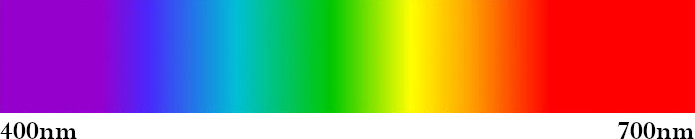
\includegraphics[width=\textwidth]{img/espectro-visible.jpg}
    \caption{Espectro de luz visible}
    \label{fig:espectro-luz-visible}
\end{figure}

Si se toman los colores primarios que aparecen dentro del espectro de luz visible (rojo, verde y azul) y se superponen para crear una combinación de estos mismos, se puede recrear cualquier otro color que se muestra en el rango del espectro. El resultado de esta operación genera el modelo de colores \textbf{CIE RGB}:

\begin{figure}[!ht]
    \centering
    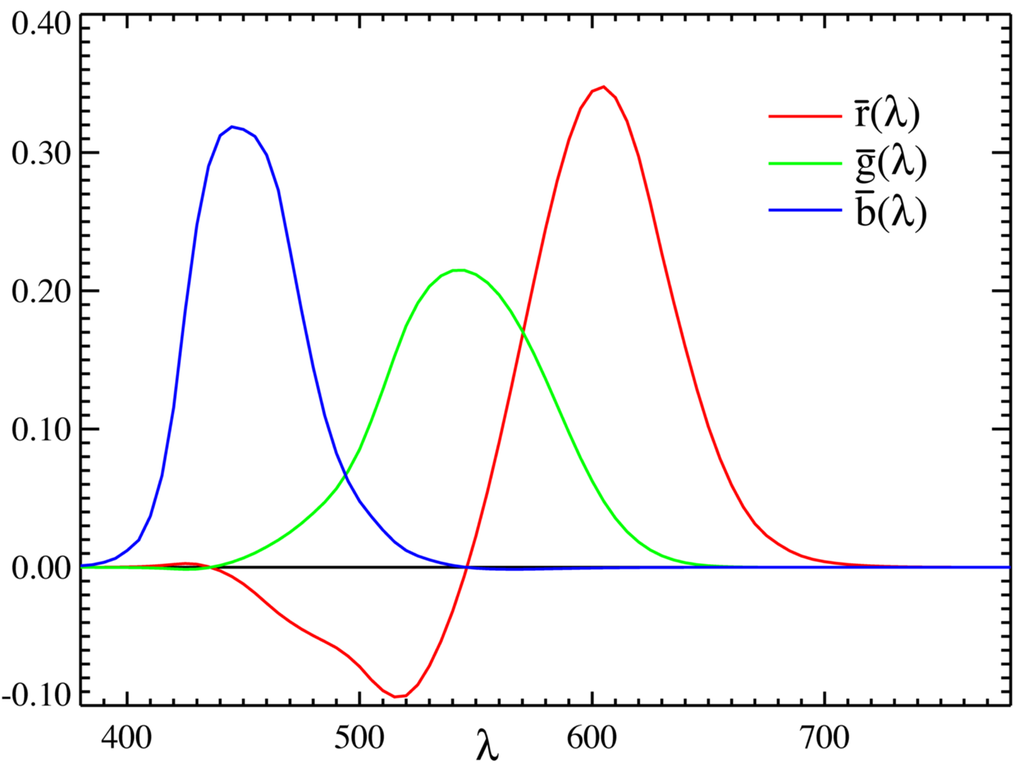
\includegraphics[width=0.5\textwidth]{img/cie-rgb.png}
    \caption{Modelo de color CIE RGB}
    \label{fig:modelo-cie-rgb}
\end{figure}

Este modelo tiene la particularidad de que el color rojo tiene un rango de valores en los que su intensidad es negativa, esto podría causar errores y dificultades para la manipulación de imágenes, por lo que el modelo \textbf{CIE XYZ} implementa una solución para este problema, aplicando un mapeado del modelo utilizando una transformación de forma que los parámetros $r$, $g$, y $b$ puedan tener solamente rangos de valores positivos:

\begin{figure}[!ht]
    \centering
    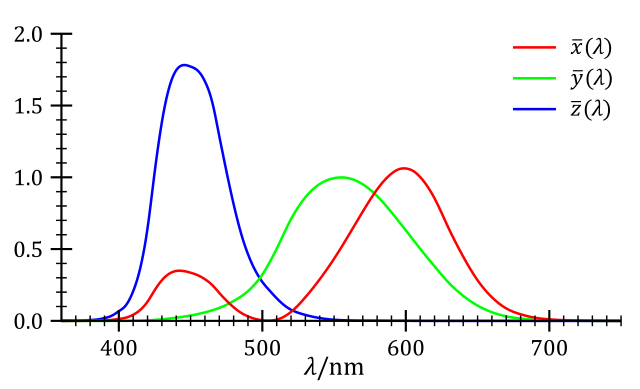
\includegraphics[width=0.5\textwidth]{img/cie-xyz.png}
    \caption{Modelo de color CIE XYZ}
    \label{fig:modelo-cie-xyz}
\end{figure}

\section{Histograma de una imagen y filtros}
El \emph{histograma de una imagen} es una gráfica que representa el rango de valores que puede tomar cada pixel de una imagen:

\begin{figure}
    \centering
    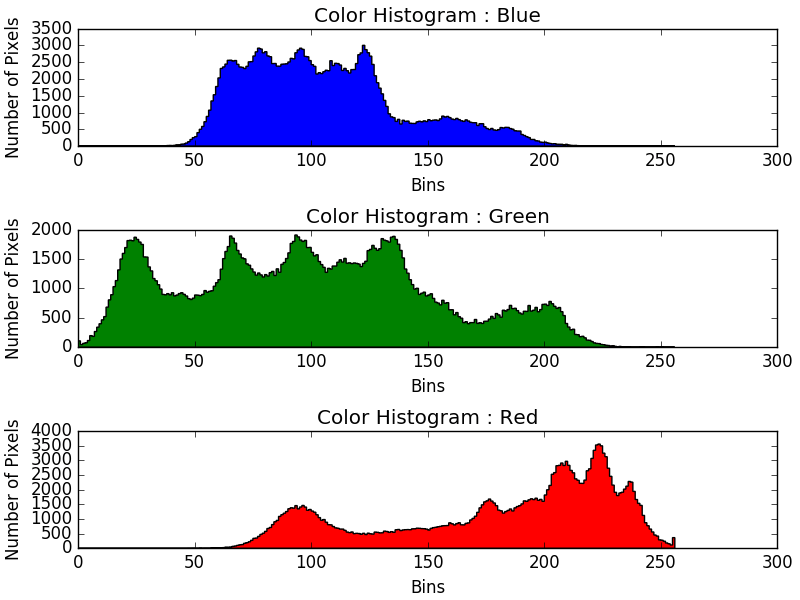
\includegraphics[width=0.5\textwidth]{img/histograma-rgb.png}
    \caption{Histogramas Red-Green-Blue de una imagen}
    \label{fig:histogramas-rgb}
\end{figure}

La información más común que puede representarse en el histograma es la cantidad de pixeles que utilizan cierta intensidad de Rojo, Verde, o Azul. Este histograma puede modificarse de forma que afecte la apariencia inicial de una imagen, esta manipulación comúnmente se le conoce como \textbf{filtro}.

Un filtro también se conoce como una \emph{máscara} o matriz que puede aplicarse en ciertas zonas de la matriz de una imagen para alterar la apariencia visual final de la misma. Para este reporte se carga una imagen aplicando una máscara que convierte los píxeles de la imagen a adquirir rangos de valores neutrales para que aparezca en blanco y negro.

\section{Procesamiento de una imagen}
Para demostrar el procesamiento digital de una imagen, se utiliza la librería OpenCV dentro de un ambiente de Anaconda con Python. Las 2 tareas principales de este procesamiento es convertir la imagen a una gama de color en blanco y negro, después realizar una transformación de rotación de 60 grados.

Primeramente para cargar la imagen al programa se importa la librería de OpenCV y se define la variable \lstinline{img} en la cual se almacena la información de la imagen \lstinline{dog.jpg} con la función \lstinline{imread()}:

\begin{lstlisting}
    import cv2 as cv
    img = cv.imread('dog.jpg')
\end{lstlisting}

Posteriormente, se reasigna la variable \lstinline{img} al retorno de la función \lstinline{cvtColor()} (\emph{Convert-Color}) la cual toma como parámetro la misma variable \lstinline{img}, y el modelo de color que se aplicará a la imagen, en este caso el modelo es \lstinline{COLOR_BGR2GRAY} para convertir la gama a escala de grises:

\begin{lstlisting}
    img = cv.cvtColor(img, cv.COLOR_BGR2GRAY)
\end{lstlisting}

Después, para aplicar una transformación de rotación se deben obtener las dimensiones de la imagen y su centro para tomarlo como punto de referencia para realizar la rotación:

\begin{lstlisting}
    (h, w) = img.shape[:2]
    (cX, cY) = (w // 2, h // 2)
\end{lstlisting}

\lstinline{(h,w)} son las dimensiones de la imagen (alto y ancho), \lstinline{(cX,cY)} es el par de coordenadas del centro de la imagen. Para generar la matriz de rotación se utiliza la función \lstinline{getRotationMatrix2D()} dados el centro de la imagen, el grado de rotación y el escalamiento, posteriormente se aplica a la imagen con la función \lstinline{warpAffine()} la cual como parámetros toma la imagen (\lstinline{img}), la matriz de transformación (\lstinline{M}), y las dimensiones (\lstinline{(w,h)}):

\begin{lstlisting}
    M = cv.getRotationMatrix2D((cX, cY), 60, 1.0)
    img = cv.warpAffine(img, M, (w, h))
\end{lstlisting}

Finalmente, para mostrar el resultado final de aplicar la transformación y el filtro se utiliza la función \lstinline{imshow()}:

\begin{lstlisting}
    cv.imshow('B&W + 60deg', img)
\end{lstlisting}

La siguiente figura muestra la imagen original y la imagen con la transformación y el filtro:

\begin{figure}[!ht]
    \centering
    \begin{subfigure}[b]{0.3\textwidth}
        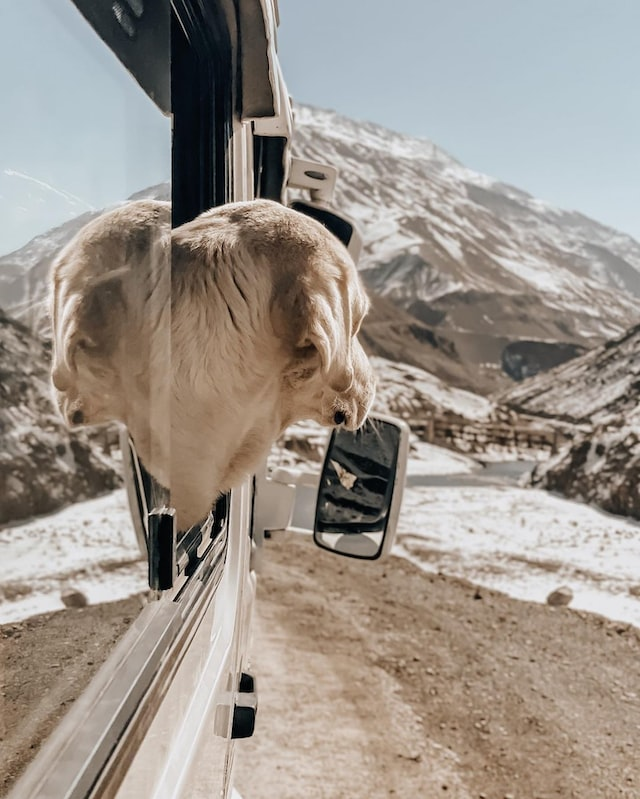
\includegraphics[width=\textwidth]{img/dog.jpg}
        \caption{Original}
        \label{fig:imagen-original}
    \end{subfigure}
    \hfill
    \begin{subfigure}[b]{0.3\textwidth}
        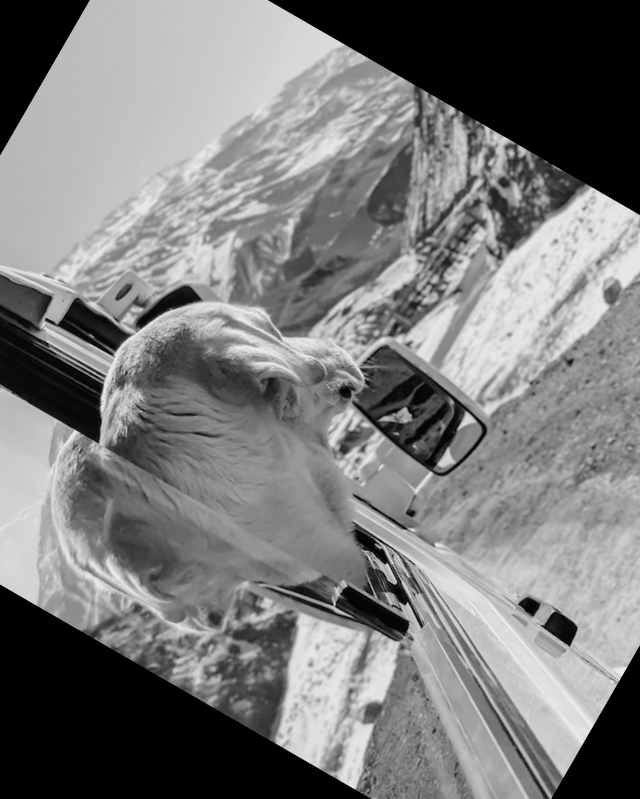
\includegraphics[width=\textwidth]{img/dog-transformed.png}
        \caption{Transformada}
        \label{fig:imagen-transformada}
    \end{subfigure}
    \caption{Imagen original vs Imagen transformada}
    \label{fig:imagenes}
\end{figure}

\bibliographystyle{plain}
\bibliography{refs}
\nocite{*}
\end{document}